% \chapter{Integrating mechanical computation into custom objects}
%\chapter{Processing digital signals}
\chapter{Digital mechanical metamaterials}
\label{chapter:digital}

% \todo{
% similar to our work on digital, based on \\
% Zanaty2018: Programmable Multistable Mechanisms: Synthesis and Modeling\\
% Merkle1993: Two Types of Mechanical Reversible Logic
% }

% \todo{add to DIGITAL for recharging: Wu2018 - Metastable modular metastructures for on-demand reconfiguration of band structures and nonreciprocal wave propagation}


% \todo{write transition from talk: stiffnes ratio, decay, ...}


% Personal fabrication machines, such as 3D printers, allow users to make custom objects. While early work on 3D printing revolved around designing the outside of such objects [24, 32], recently researchers started exploring 3D printing as a means to design the \textit{inside} of objects. Applications include moving objects’ centers of gravity so as to make them stand [20] or spin [1].

% Pushing this further, researchers created objects that consist internally of a large number of 3D cells arranged on a regular grid [15]. Since each cell is designed to perform a specific deformation, objects that entirely consist of such cells literally offer thousands of degrees of freedom. Such structures are also known as \textit{metamaterials} [18].

% While metamaterials were initially understood as materials, we recently proposed to think of them as \textit{machines}; such metamaterial mechanisms [10] consist of a single block of material, the cells of which play together in a well-defined way in order to achieve macroscopic movement. We used this principle previously to implement simple mechanical objects, such as a door latch (\todo{Figure 7}).

Metamaterial mechanisms, like all \textit{analog} machines, are limited in terms of complexity. As forces are passed on from one cell to the next, they are damped and the activation energy dissipates, which causes the mechanical ``signal" to decay exponentially. This limits the number of mechanisms that can be concatenated and therefore the complexity of the machine.

In this work, we explore how to extend this concept towards \textit{digital} mechanisms. Combining metamaterial mechanisms with concepts from mechanical computing and mechanical signal propagation \cite{Raney2016, Nadkarni2014}, we introduce a new type of cell that propagates a digital mechanical signal, i.e., it counteracts signal decay and thus allows signals to pass through an arbitrary number of cells. We extend this basic mechanism to implement simple logic functions. 

To illustrate this concept, Figure \ref{fig:1-door-lock} shows a combination lock implemented using digital metamaterials. The device offers ten digit buttons on the front. Users tap these buttons to enter their code, then press the `open' button to unlock the door. 

\begin{figure} [h]
    \includegraphics[width=\textwidth]{chapters/digital-metamaterials-FIG/1-door-lock.pdf}
    \caption[Short figure name.]{(a) This combination door lock is implemented as a \textit{digital mechanical metamaterial}, i.e., a single block of material based on a regular grid of cells. It allows users to input a numeric code, it processes the code, checks its correctness, and unlocks the latch. (b) Under the hood, the lock consists of an array of cells that transmit and process a mechanical signal. 
    \label{fig:1-door-lock}}
\end{figure}


\section{Basic cells of digital mechanical metamaterials}

Digital metamaterials are based on a new type of cell that propagates a mechanical signal reinforced by an embedded bistable spring. 


\subsection{The bit cell is the main underlying mechanism}

Figure \ref{fig:2-bit-cell} shows the key element behind digital metamaterials, which we call \textit{bit cell.} Bit cells contain a bistable spring, which allows them to take on two discrete states. Figure \ref{fig:2-bit-cell}a shows the bit cell in its \textit{tense state.} (b) When triggered, the spring discharges, causing the cell to switch from its \textit{tense} state to its \textit{relaxed} state.  

\begin{figure} [h]
    \includegraphics[width=\textwidth]{chapters/digital-metamaterials-FIG/2-bit-cell.pdf}
    \caption[Short figure name.]{(a) When triggered, this \textit{bit cell} changes its state from tense to (b) relaxed.
    \label{fig:2-bit-cell}}
\end{figure}

As shown in Figure \ref{fig:3-ports-at-cell}, bit cells feature an input port and output port. A mechanical impulse that reaches the input port triggers the cell, which creates an impulse at the output port. Because discharging the spring releases mechanical energy, the impulse at the output port is larger than the required trigger impulse at the input port.

\begin{figure} [h]  
    \includegraphics[width=\textwidth]{chapters/digital-metamaterials-FIG/3-ports-at-cell.pdf}
    \caption[Short figure name.]{Bit cells offer an input and an output port.
    \label{fig:3-ports-at-cell}}
\end{figure}

As illustrated by Figure \ref{fig:4-signal-transmission}, this allows us to concatenate bit cells in a way that allows cells to trigger their immediate neighbors, resulting in a simple signal propagation mechanism similar to \cite{Raney2016}.

\begin{figure} [h]  
    \includegraphics[width=\textwidth]{chapters/digital-metamaterials-FIG/4-signal-transmission.pdf}
    \caption[Short figure name.]{Concatenating bit cells creates a signal transmission. (a) Initially all bit cells are in their tense position. (b) Triggering the leftmost cell causes the signal to propagate through all cells from left to right.
    \label{fig:4-signal-transmission}}
\end{figure}

\subsection{The combination lock example}

Bit cells and the resulting concept of signal propagation allow us to implement a hierarchy of digital mechanisms of increasing complexity. We discuss these logic functions and mechanisms in full detail later in this paper, as well as a simple manual recharge mechanism to set discharged springs back into their tense state. However, Figure \ref{fig:5-elements-in-the-door-lock} provides a rough overview of the different elements that implement the combination lock.

\begin{figure} [h]  
    \includegraphics[width=\textwidth]{chapters/digital-metamaterials-FIG/5-elements-in-the-door-lock.pdf}
    \caption[Short figure name.]{Our door lock consists of 82 cells, which implement the signal transmisison, the evaluation of each digit input by the user, an AND gate, and one amplifier cell with a pre-amplification step to move the blocking bolts sufficiently.
    \label{fig:5-elements-in-the-door-lock}}
\end{figure}

(1) To input the code, users tap one of the digit buttons on the front, which changes the state of the \textit{digit evaluation} cells. The device contains 10 of these---one for each possible digit. (2) When the user pushes the `open' button, three signal transmission lines are set off simultaneously; two of which run through the digit evaluation units and (3) set the state of the \textit{AND gate.} The AND gate evaluates the correctness of the code by computing a logical AND the two rows of digits input by the user. The third signal transmission line runs from the bottom left towards the right, around the corner, and upwards where (4) the signal is \textit{bifurcated.} This allows triggering (5) a double-sized \textit{amplifier cell} that actuates the bolts to unblock the door.

Figure \ref{fig:6-bolts} shows a close-up of these bolts. (a) As long as the bolts are in place, they prevent the shearing cells in the middle from shearing, thereby blocking the door. (b) When the bolts are retracted, the shearing cells can shear and pushing down the handle retracts the latch---as we discussed in Chapter \ref{chapter:analog-metamaterials}. This is where our digital metamaterials connect to the analog metamaterial door latch mechanism.

\begin{figure} [h]  
    \includegraphics[width=\textwidth]{chapters/digital-metamaterials-FIG/6-bolts.pdf}
    \caption[Short figure name.]{We effectively lock the latch mechanism by stiffening the shearing area that enables it. We do so by inserting bolts. Once users entered the key code correctly, our lock signal retracts the bolt and enables the latch mechanism.
    \label{fig:6-bolts}}
\end{figure}


\section{Contribution, benefits and limitations}

Our main contribution is the concept of digital mechanical metamaterials. They allow integrating computational abilities into the structure of 3D printed objects. We provide a modular system consisting of digital cells (hardware) and an editor (software) that provides a toolkit to users, enabling them to create new digital mechanisms. 

While analog metamaterial mechanisms are subject to damping, which causes the mechanical ``signal" to decay exponentially and limits the number of `steps' that can be performed, \textit{digital} mechanical metamaterials enable transmitting signals through an \textit{arbitrary} number of cells. 

When we contrast digital mechanical metamaterials to the traditional approach of augmenting objects with electronic microcontrollers, sensors, and actuators \cite{Savage2014}, our approach results in an entirely mechanical solution and can be produced entirely using a 3D printer. However, since our approach lacks loops, clocks, and memory, our approach is limited to much simpler devices.


\subsection {Scope of this concept}
% \todo{add scope to set expectations right: schaltnetz vs schaltwerk, is turing complete?}

This work, more than the other works in this thesis, is a thought experiment, a what-if question, rather than a potential solution to a potential problem. Our digital metamaterials are by no means intended to replace computers. We aimed to investigate the question, whether the habit of using microcontrollers for very simple evaluation or computations is really necessary, or if we can perform simple operations within the metamaterial structure.  

The scope of our current implementation spans \textit{combinational circuits} (ger. Schaltnetz). Our cell-based material can perform any combinational logic, as we will demonstrate a NAND gate in Section \ref{section:digital-gates}. Furthermore, like combinational circuits our metamaterials present time-independent logic, i.e., the output is a pure function of the present input only.

This work could be expanded to sequential circuits (ger. Schaltwerk) by engineering a protected region that is unaffected by the recharging action and can thus act as memory, and by introducing an external clock signal. 



\section{Signal processing based on cells}

\subsection{Routing signals}

In this and the following section, we now show the individual cells that implement the combination door lock we showed in Figure \ref{fig:5-elements-in-the-door-lock}. We begin with the cell types that allow us to route signals through 3D objects. We already looked at signal propagation along a straight line (Figure \ref{fig:4-signal-transmission}); in this section, we demonstrate how to route signals around corners, across other signal lines, and how to bifurcate signals. 

Routing signals is important because 3D printed objects can have arbitrary shape and routing allows transmitting a signal from where it emerges to where the information is needed. For the door lock, for example, we route users input from the digit inputs to the door latch mechanism---which is located elsewhere in our object.

The more specialized routing cells are all based on \textit{bit cells.} However, we position their output ports to be oriented towards the neighbor cell we want to trigger. So while the bit cells in Figure \ref{fig:4-signal-transmission} feature an output port on the side opposite to the input port, the cell shown in Figure \ref{fig:8-simulation-tear-and-rotate} redirects the signal by 90° by adding a beam to the arm of our bistable spring. This beam rotates with the arm of the spring, allowing it to tap the input port of the rotated cell on the top right.

\begin{figure} [h]  
    \includegraphics[width=\textwidth]{chapters/digital-metamaterials-FIG/8-signal-redirecting-90deg-2D.pdf}
    \caption[Short figure name.]{We use a new type of output port to redirect the signal by 90°. We exploit the rotational movement of the spring and attach a beam that taps its neighboring cell.
    \label{fig:8-signal-redirecting-90deg-2D}}
\end{figure}

As illustrated by Figure \ref{fig:9-siganl-redirecting-90deg-3D}, we can route signals in 3 dimensions by concatenating multiple such mechanisms. Here we route the signal from the x/y plane to the x/z plane to the y/z plane. 

\begin{figure} [h]  
    \includegraphics[width=\textwidth]{chapters/digital-metamaterials-FIG/9-siganl-redirecting-90deg-3D.pdf}
    \caption[Short figure name.]{(a) Rotating the receiving cell allows us to redirect signals from one plane to another. (b) Concatenating three assemblies allows us to route signals in 3D. 
    \label{fig:9-siganl-redirecting-90deg-3D}}
\end{figure}

Figure \ref{fig:10-signal-crossing} shows a specialized three-cell mechanism that allows two signals to pass each other in minimal space. We use a crossbar that reaches from the output port of the left cell to the input port of the right cell that spans across the middle cell.

\begin{figure} [h]  
    \includegraphics[width=\textwidth]{chapters/digital-metamaterials-FIG/10-signal-crossing.jpg}
    \caption[Short figure name.]{We cross signals by running a crossbar across another cell.
    \label{fig:10-signal-crossing}}
\end{figure}

Figure \ref{fig:11-signal-bifurcation} shows two mechanisms that bifurcate signals. The design shown in (a) triggers two parallel signal lines. The design shown in (b) triggers two signal lines oriented in opposite directions. Both designs exploit the fact that our bistable springs require less energy to be triggered than they output, which allows triggering two cells from one. 

\begin{figure} [h]  
    \includegraphics[width=\textwidth]{chapters/digital-metamaterials-FIG/11-signal-bifurcation.pdf}
    \caption[Short figure name.]{We can bifurcate signals (a) in a parallel manner or (b) let the two signals run in opposite directions. 
    \label{fig:11-signal-bifurcation}}
\end{figure}

Figure \ref{fig:12-signal-merging-OR} shows how we merge two signals. This is an interesting construct, because it implements an OR gate.

\begin{figure} [h]  
    \includegraphics[width=\textwidth]{chapters/digital-metamaterials-FIG/12-signal-merging-OR.jpg}
    \caption[Short figure name.]{We use the opposite assembly to merge signal as we did to bifurcate them. This implements an OR gate.
    \label{fig:12-signal-merging-OR}}
\end{figure}


\subsection{Logic functions}

To implement logic functions, we need to go beyond merely transmitting signals to also evaluating signals, which we achieve by blocking them. In the combination lock from Figure \ref{fig:5-elements-in-the-door-lock}, we block signals for wrong digit inputs so that the door stays blocked. Later in this section, we present cell arrangements that implement basic logic, such as AND or NAND.

\subsubsection{Blocking signals using gate cells}

To allow for asynchronous input, we have designed cells capable of storing the first input that reaches them and do not act until the last signal has been received. We call these cells \textit{gate cells.} Our approach is based on rod logic \cite{Merkle1993}. 

As illustrated by Figure \ref{fig:13-gate-cells-illustration}a these cells work by placing a ``blocker" across their neighboring cell. When the cell on the right is triggered before the cell on the left, the blocker is aligned with the output port of the right cell so that it cannot pass and signal is blocked. However, triggering the left cell, as shown in Figure \ref{fig:13-gate-cells-illustration}b, moves the blocker out of the way and the signal can pass through. The position of the blocker can also be defined to initially let signals through and only after actuation to block signals, as shown in Figure \ref{fig:13-gate-cells-illustration}c-d.

\begin{figure} [h]  
    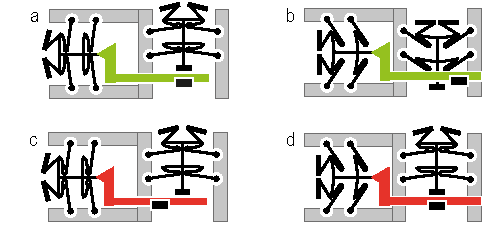
\includegraphics[width=\textwidth]{chapters/digital-metamaterials-FIG/13-gate-cells-illustration.pdf}
    \caption[Short figure name.]{\textit{Gate cells} validate signals and can be configures to block signals (a-b) or let signals pass (c-d) in their tense state.
    \label{fig:13-gate-cells-illustration}}
\end{figure}

Figure \ref{fig:14-signal-blocking} shows the design of the two cells that form the gate cell. Each crossbar has a blocker attached on its underside.

\begin{figure} [h]  
    \includegraphics[width=\textwidth]{chapters/digital-metamaterials-FIG/14-signal-blocking.JPG}
    \caption[Short figure name.]{We position a blocking element that is intended to either block the signal output or let it pass.
    \label{fig:14-signal-blocking}}
\end{figure}


\subsubsection{Logic functions based on gate cells}

We can concatenate multiple gate cells to create combinational logic functions. Figure 15 uses simplified symbols to illustrate how the positions of the blockers are configured to implement the function $A\ {\land}\ {\neg}B\ {\land}\ C\ {\land}\ D\ {\land}\ {\neg}E$. The positive input cells A, C, and D need to be triggered to move the blocker out of the way and let the signal pass. The negated inputs B and E are implemented by positioning the blocker so that they let the signal pass when they are \textit{not} triggered and block the signal otherwise.

If we rename the inputs of the logic function that is shown in Figure \ref{fig:15-code-evaluation-1--5} from A--E to 0--4, it implements a 5-digit code evaluation. To implement the combination lock with 10 digits, we add a second row of inputs. Now we have two logic functions (one in each row), which both need to be correct, thus we add an AND gate. Figure \ref{fig:16-code-evaluation-0--9} illustrates that the key code is `0 2 3 8'. 

\begin{figure} [h]  
    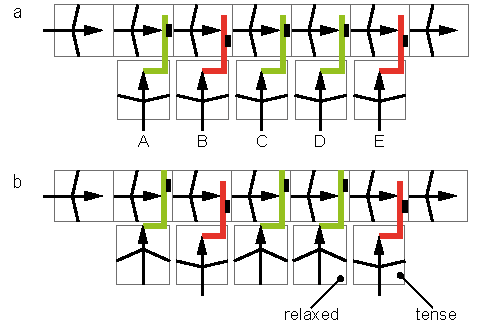
\includegraphics[width=\textwidth]{chapters/digital-metamaterials-FIG/15-code-evaluation-1--5.pdf}
    \caption[Short figure name.]{(a) When all inputs are tense, the signal cannot pass. (b) Triggering the correct inputs, here A, C, and D, moves the blockers so that the signal can pass.
    \label{fig:15-code-evaluation-1--5}}
\end{figure}

\begin{figure} [h]  
    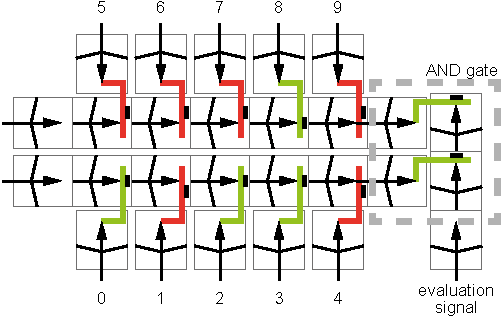
\includegraphics[width=\textwidth]{chapters/digital-metamaterials-FIG/16-code-evaluation-0--9.pdf}
    \caption[Short figure name.]{We add an AND gate to validate the two rows that yield the 10-digit.
    \label{fig:16-code-evaluation-0--9}}
\end{figure}

Again, we use our \textit{gate cells} to employ the AND gate. Each code evaluation row has a gate cell at the end. Only if all the inputs of the corresponding row were correct, the blocker is moved out of the way for a third signal to pass, the \textit{evaluation signal.} 


\subsubsection{Combinational logic using an evaluation signal}
\label{section:digital-gates}

Our implementation of the AND gate has three inputs, namely two values and one additional \textit{evaluation signal.} We add this additional signal because our mechanical computation is fundamentally different from electronic circuits yet adding only one single signal allows us to implement any Boolean predicate without any electronics. 

A `signal' within our system is not an applied voltage, but an \textit{impulse,} i.e., a mechanical force within the object. This impulse \textit{changes the system state} by changing physical properties of the material, such as the position of the blockers. Since we block invalid signals, the output of gate cells is no signal instead of a 0-signal (logical low). However, not receiving a signal is indistinguishable from a dormant system. This means that we cannot provide an 0-signal that can serve as an input to the next gate, as in classical electronic circuits.

Despite this, we are still able to employ combinational logic within our materials. The most space efficient way is to integrate the inversion into logic functions, e.g., by using a NOR instead of an OR. Figure \ref{fig:17-gates} illustrates a selection of logic gates implemented with our digital cells. Note that we show a different OR gate compared to the one shown in Figure \ref{fig:12-signal-merging-OR}. The one shown here uses the general-purpose assembly that is also used in the NOT and NAND gate. 

\begin{figure} [h]  
    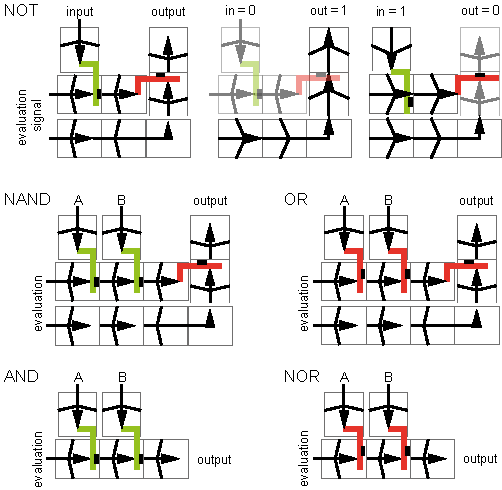
\includegraphics[width=\textwidth]{chapters/digital-metamaterials-FIG/17-gates.pdf}
    \caption[Short figure name.]{Only one additional signal allows us to implement combinational logic, despite not having a traditional 0-signal.
    \label{fig:17-gates}}
\end{figure}

We add the additional evaluation signal as a second computation step. After the inputs are provided to the system, we send a signal off that evaluates the inputs in order to produce output. Independent of the complexity of the logic, only one single evaluation signal is necessary, since it can be furcated, merged, and routed through the material. Race conditions within operations can be resolved by adapting the length of signal paths.


\subsection{Amplifying the output}

While the cells that implement the signal transmission can be arbitrarily small, the \textit{output} cells that move material to change the material properties might need to produce a certain amount of movement or force.

In the example of the door lock, we need to move the bolts sufficiently far into the door latch's structure to stiffen it. We use what we call an \textit{amplifier cell,} which is inspired by the metaphor of operational amplifiers in the electronics domain. Such an amplifier cell, as shown in Figure \ref{fig:18-amplify-signal}, is a cell that is doubled in size. This allows us to add a larger spring to produce more stroke length.

\begin{figure} [h]  
    \includegraphics[width=\textwidth]{chapters/digital-metamaterials-FIG/18-amplify-signal.jpg}
    \caption[Short figure name.]{We amplify the stroke length of our output by going from small cells to a double-sized cell. 
    \label{fig:18-amplify-signal}}
\end{figure}

To transition from small cells to bigger cells, we bifurcate the signal. This gives us the energy of two cells, which together trigger the spring within the amplifier cell. In our door lock example, our $30\, \mathrm{mm}$ amplifier cell moves the bolts by $6\, \mathrm{mm}$ as compared to the stroke length of $3\, \mathrm{mm}$ of the $15\, \mathrm{mm}$ bit cells.


\subsection{Recharging}

After the springs were triggered and they are in their relaxed state, they need to be reset to their tense state before the computation can be run again. To do so, we designed a small lid on top of each cell, which uses the cell's third dimension to recharge the spring. Figure \ref{fig:19-recharging-OR__TEMP} shows how as the lid is pushed down, the attached wedges move the spring backward to its tense position. We use an additional plate to push multiple recharge lids at the same time. This design enables one recharge action for every plane of computation. We added a small bump on the underside of the lid, which causes the lid to spring back upward in order to not hinder the signal transmission between the cells.

\begin{figure} [h]  
    \includegraphics[width=\textwidth]{chapters/digital-metamaterials-FIG/19-recharging-OR__TEMP.png}
    \caption[Short figure name.]{(a) Each cell features a lid with wedges, pushing it (b) recharges the spring underneath.
    \label{fig:19-recharging-OR__TEMP}}
\end{figure}


\subsection{Scope of Applications}

We see digital mechanical metamaterials being particularly useful for objects that have (1) many mechanical inputs (e.g., the code lock), and/or (2) many mechanical outputs (e.g., the following example of a plant pot), and (3) which are not frequently reconfigured. For example, the density plant pot might be reconfigured when seasons change, or the door might be locked once a day. In contrast, for objects that require frequent updates (e.g., displays) or more complex programming involving loops, etc., we recommend traditional electronics. 

\subsubsection{Additional example: plant pot}

Figure 20 shows an example of a plant pot, where (a) users input the plant’s size (small--large) and its water demands (little--much) using sliders. This triggers the computation in the bottom layer of the pot, which determines (b) how many \textit{density cells} will be closed. After users configured the pot's density, (c) they place it into a cachepot with water. The density of the plant pot now determines how fast water can pass through to the plant. 

\begin{figure} [h]  
    \includegraphics[width=\textwidth]{chapters/digital-metamaterials-FIG/20-plant-pot-walkthrough-combined.pdf}
    \caption[Short figure name.]{We implement a plant pot that changes its density based on user input of the plant's size and water demands. 
    \label{fig:20-plant-pot-walkthrough-combined}}
\end{figure}

We use \textit{gate cells} to change the weight of the parameters of the plant pot example. Figure \ref{fig:21-plant-pot-logic} shows that by simply placing gate cells along the diagonal, we give more weight to the low values of the parameters. Since the gate cells prevent the signal from passing through, they prevent all density cells from closing, so that even for a small plant with little water demand the plant pot’s permeability is 25\% (3 out of 12 density cell rows remain open).

\begin{figure} [h]  
    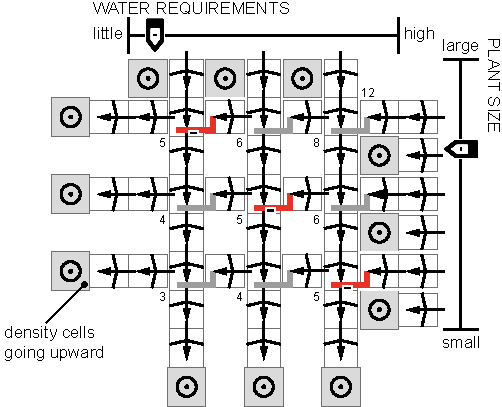
\includegraphics[width=\textwidth]{chapters/digital-metamaterials-FIG/21-plant-pot-logic.pdf}
    \caption[Short figure name.]{The weighted computation of the plant pot's density ensures that small plants get enough water by preventing some density cells from closing. The numbers indicate how many density cells are open for each parameter combination.
    \label{fig:21-plant-pot-logic}}
\end{figure}


\section{Technical detail on the cells}

\subsection{Fabrication of cells}

We print our prototypes from the commonly available filaments ABS and PLA. While our cells are designed to be printed in an assembled state, we tend to print the parts of our prototypes separately. This allows us to print all elements without support material, which tends to be faster than the single-part design that requires dissolving the support material. We printed the springs from PLA using the \textit{Ultimaker 2+} 3D printer, and the frames that hold the springs from ABS on our \textit{Stratasys Dimension SST 1200es.} Our cell size is $15\, \mathrm{mm}$ for all our prototypes with a printed spring thickness of $0.4\, \mathrm{mm}$.

The cell shown in Figure \ref{fig:22-cell-printed-assembled} is printed in an assembled state. We had it made at \textit{shapeways} using their ``frosted detail plastic" material, which is a UV cured acrylic polymer that is printed using the MultiJet Modeling process. 

\begin{figure} [h]  
    \includegraphics[width=\textwidth]{chapters/digital-metamaterials-FIG/22-cell-printed-assembled.jpg}
    \caption[Short figure name.]{A cell printed fully assembled using shapeways' ``frosted detail plastic" material. 
    \label{fig:22-cell-printed-assembled}}
\end{figure}

We empirically tested how the cells miniaturize while retaining the same stress values using \textit{Autodesk Fusion's} simulation. The results showed that reducing the spring thickness to \(\frac{1}{2}\) allows it to be shortened to \(\frac{1}{4}\) of its length, i.e., to \(\frac{1}{64}\) of the cell volume. For example, a $0.2\, \mathrm{mm}$ thick spring allows for a cell size of $3.75\, \mathrm{mm}$, which is a matter of printer resolution.


\subsection{Bistable spring design}

The bistable spring in our cells differs from a typical bistable spring that is shown in Figure \ref{fig:23-springs-simple-vs-ours}b, which is a simple pre-bent beam that is fixed within rigid walls \cite{Qiu2004}. However, such designs have very high width-to-length ratios, which do not utilize the space within a rotation-invariant cubic cell well.

\begin{figure} [h]  
    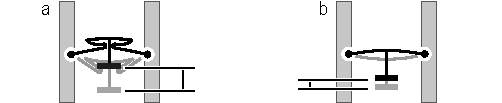
\includegraphics[width=\textwidth]{chapters/digital-metamaterials-FIG/23-springs-simple-vs-ours.pdf}
    \caption[Short figure name.]{(a) The spring we use in our bit cells is longer and thus weaker than (b) conventional bistable springs. Or, for the same force, our cells produce more stroke length.
    \label{fig:23-springs-simple-vs-ours}}
\end{figure}

Figure \ref{fig:23-springs-simple-vs-ours} illustrates that our spring design includes an additional `loop', which prolongs the beam and therefore makes it weaker, i.e., it requires less force to be triggered and charged. We measured 45\% less force required to charge our type of spring compared to the conventional spring. Another way to view it is that our longer springs produce more output length (by 23\% according our measurements) while requiring similar force. 

Note that our cells incorporate two connected springs. This is a common technique \cite{Qiu2004} for increasing the stability of bistable springs during the so-called `snap-through', i.e., the point where the spring is compressed the most as it is forced to its other second position. 


\subsection{Technical evaluation}

The geometry of our spring allows us to make limited changes in stroke length and force by varying the spring parameters. For example, we used slightly stronger springs in the plant pot example to compensate for the higher density of water. While the output of bit cells usually needs to be only strong and far enough to trigger the neighbor cell, the output cells may have to meet specific requirements in terms of amount of force or stroke length.

Our evaluation informs the geometrical spring parameters for achieving bistability and the maximum possible fan-out of a cell, i.e., how many cells can be triggered by one single cell.

\paragraph{Independent variables.} We compared a total of 75 springs of our design where we varied three parameters independently illustrated by Figure \ref{fig:24-spring-details}: (1) the arm angle, (2) the length of the bent bridge in the middle, and (3) the strength of the bridge, varied trough changing its buckling magnitude and its thickness concurrently. We varied the values for the bridge strength from $1.05 \times$ the normal spring thickness to $1.85 \times$, and a buckle distance from 8\% of the bridge length to 40\%. The spring thickness is limited by the 3D printer’s resolution; we use $0.18\, \mathrm{mm}$. Bridge length values ranged from 45\% to 85\% the total distance between the walls. We tested these values for 20°, 30° and 40° arm angles. This yields 25 springs for each arm angle.

\begin{figure} [h]  
    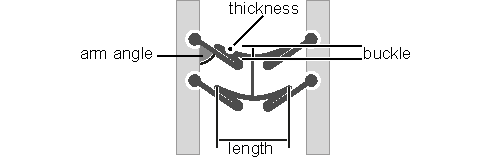
\includegraphics[width=\textwidth]{chapters/digital-metamaterials-FIG/24-spring-details.pdf}
    \caption[Short figure name.]{We vary the parameters of bridge length and bridge strength for three different arm angles each. We measure the stroke length and the forces for charging and triggering the springs, as well as their output energy.
    \label{fig:24-spring-details}}
\end{figure}

\paragraph{Dependent variables.} We measured (1) the force it takes to push a spring to its tense position, (2) the force necessary to trigger the spring, (3) its stroke length, and (4) the force it outputs when triggered. 

\paragraph{Test setup.} Figure \ref{fig:25-measurement-setup} shows our test setup. We placed a ruler (error $0.5\, \mathrm{mm}$) under the spring to measure the stroke length. We used a force gauge with an error of $0.05\, \mathrm{N}$, which was constrained to linear movement centered to the spring and precisely moved by a threaded rod. We pushed the force gauge against the spring to measure the charge energy, we released the pressure while slowly moving the force gauge backward to measure the output energy, and we measured the trigger energy by pushing the rotated spring.

\begin{figure} [h]  
    \includegraphics[width=\textwidth]{chapters/digital-metamaterials-FIG/25-measurement-setup.jpg}
    \caption[Short figure name.]{We measure the forces using a force gauge (error $0.05\, \mathrm{N}$), and the stroke length using a ruler (error $0.5\, \mathrm{mm}$).
    \label{fig:25-measurement-setup}}
\end{figure}

\subsection{Results}

Figure \ref{fig:26-results} shows charge, output, and trigger energy and stroke lengths for 50 springs. Empty fields denote springs that were not bistable. The results for springs with a 20° arm angle were omitted since only 2 of them were bistable. 

All four measured values increase when increasing the arm angle or the bridge strength, or when decreasing the length of the bridge. The \textit{output energy} was on average 73\% of the charge energy for 30° springs and 66\% for 40° springs. 

The difference between output energy and \textit{trigger energy} is greatest right when the springs start becoming bistable. The ratio between the two decides the maximum possible fan-out of the springs, thus a 2:1 ratio is necessary for bifurcation. Choosing a higher trigger energy however increases the fault-tolerance of the system with regards to unwanted activation, e.g., by dropping the object. 

\begin{figure} [!h]  
    \centering
    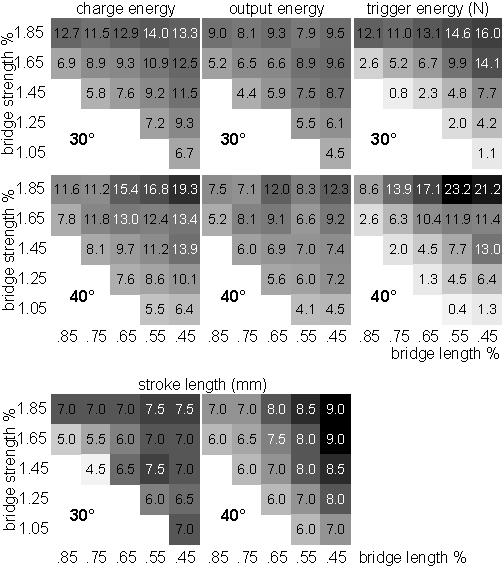
\includegraphics[width=\textwidth]{chapters/digital-metamaterials-FIG/26-results.pdf}
    \caption[Short figure name.]{Raw results of our technical evaluation for charge, output and trigger energy in $\mathrm{N}$ and stroke length in $\mathrm{mm}$. Missing values indicate non-bistable springs.
    \label{fig:26-results}}
\end{figure}

\textit{Stroke length} is affected most by the arm angle, i.e., the stroke length increases with the arm angle. Stroke is least affected by the strength of the bridge. 

In contrast, \textit{charge energy} of the spring is affected most by the strength of the bridge and least by the arm angle, which can also be seen from Figure \ref{fig:26-results} in the rapid changes along the y-axis. 

Choosing appropriate values for each can tune the spring toward a longer stroke or a higher output energy without changes to its bistability. Note that these values apply to the springs we tested with and that due to differences in manufacturing they might vary slightly.


% \section{Editor}

% To allow expert users to create and fabricate objects from digital metamaterials, we implemented a specialized 3D voxel-style editor, which is based on the editor for metamaterial mechanisms shown in Section \ref{section:mechanisms-editor}. The main intent is to allow users to draw signal paths and verify them within the editor (Figure \ref{fig:27-editor-interface}). We support users by allowing them to enter simple logic functions, which our editor converts to cell arrangements that implement that function.

% While the editor is built to help users design digital metamaterials efficiently, knowledge about signals and logic remains necessary, i.e., this editor is for expert users. 

% \begin{figure} [h]  
%     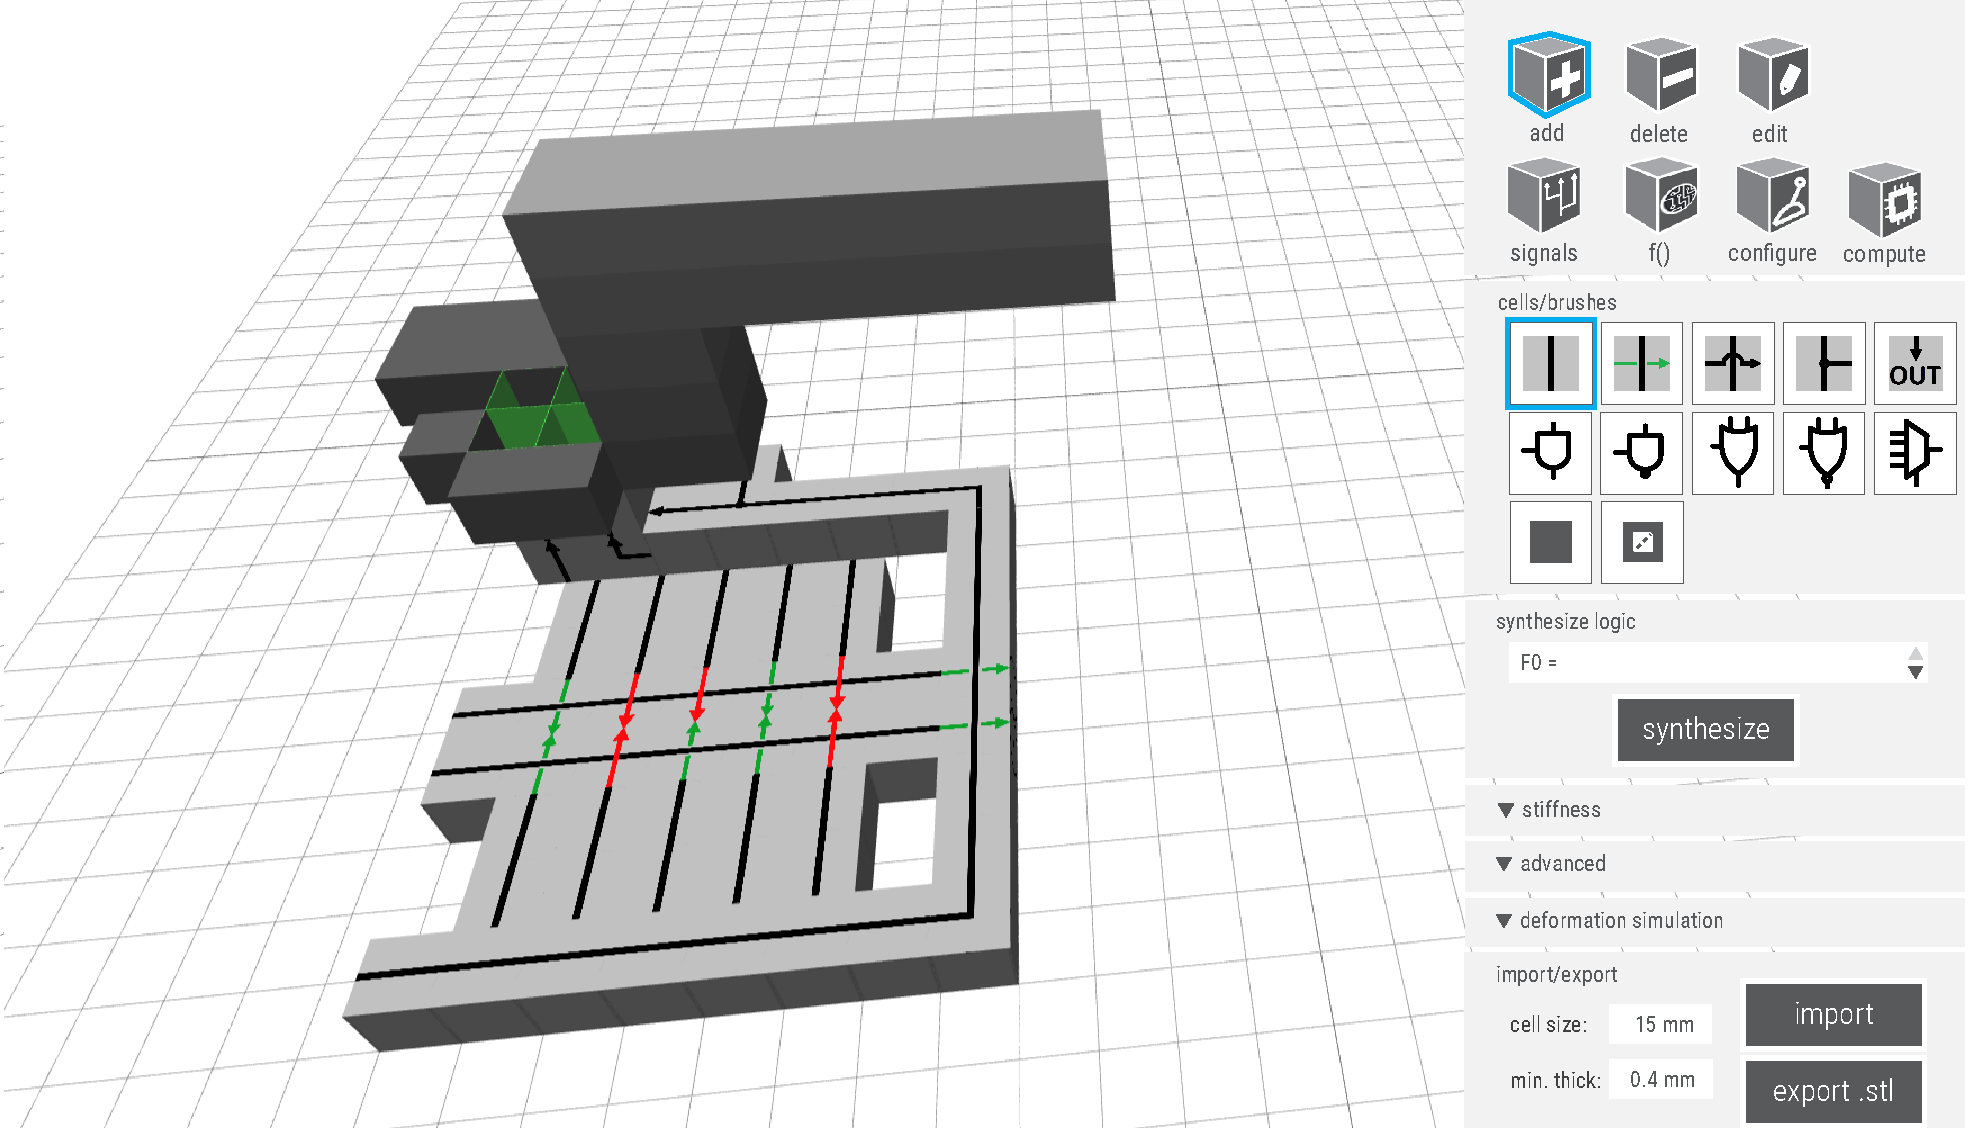
\includegraphics[width=\textwidth]{chapters/digital-metamaterials-FIG/27-editor-interface.pdf}
%     \caption[Short figure name.]{Our editor helps users create digital metamaterials.
%     \label{fig:27-editor-interface}}
% \end{figure}


% \subsection{Walkthrough}

% Figure \ref{fig:28-editor-draw-signals} illustrates how users create the door lock example from Figure 1. (a) They first draw the signal line that evaluates the upper 5 digits by dragging over the ground plane using our ``draw signals" tool. (b) Then, using the same tool, they draw signals perpendicular to the first signal line. (c) When the two signals cross, the editor automatically draws a gate cell. (d) They do the same for the lower row of digits. (e) In this example, users manually configure the gate cells using the ``configure", i.e., they change the initial state of 5 gate cells from initially `pass' to `block' by clicking on the respective gate cell. (f) The configured gate cells implement the key code for the lock. 

% Users continue by adding the evaluation line, the AND gate and the output cells, which will move the bolts. Finally, they model the analog door latch mechanism on top of the digital metamaterial. 

% \begin{figure} [h]  
%     \includegraphics[width=\textwidth]{chapters/digital-metamaterials-FIG/28-editor-draw-signals.pdf}
%     \caption[Short figure name.]{(a) Users draw the signal routing using the ``draw signals" tool. (b) Once they cross an existing signal route, (c) the editor automatically draws a gate cell. (d) After creating all cells for the digit evaluation, (e) users set the initial states of the gate cells using the ``configure" tool (f) to define the key code.
%     \label{fig:28-editor-draw-signals}}
% \end{figure}

% Figure \ref{fig:29-editor-verify-signals} shows how users verify the signal transmission in our custom editor. They first charge the cells by selecting the ``compute" tool. The editor visualizes charged cells by turning the signal lines blue. Clicking on a cell, as shown in Figure \ref{fig:29-editor-verify-signals}a, sets a signal off. The impulse runs through the cells, being visualized in yellow at the currently active cell. After the impulse has passed a cell, the signal path is shown in black again, because the cell is back in its relaxed state (Figure \ref{fig:29-editor-verify-signals}b). To verify the whole computational assembly, users trigger the inputs first and then the evaluation signal, as they do on the 3D printed object. They subsequently watch if the signal runs all the way through to the door. If not, they see where the signal stopped and can correct the error. 

% \begin{figure} [h]  
%     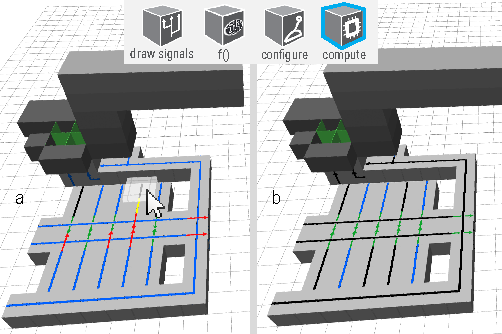
\includegraphics[width=\textwidth]{chapters/digital-metamaterials-FIG/29-editor-verify-signals.pdf}
%     \caption[Short figure name.]{Users can verify their logic and signal routing. They first charge all springs, then (a) they click the inputs to trigger the signal there, and lastly (b) they trigger the evaluation line and find that the signal passes all the way through to the latch.
%     \label{fig:29-editor-verify-signals}}
% \end{figure}

% To help users create logic functions efficiently, e.g., by avoiding the need for manual configuration of cells, we allow users to input logic functions. Figure \ref{fig:30-editor-synthesize-cells} shows an example, where users enter the function `A \& {\textasciitilde}B \& C \& D \& {\textasciitilde}E' and click ‘synthesize’. Then, they indicate where the synthesized cell arrangement shall be positioned by simply clicking on the grid. Our editor automatically synthesizes the cells that implement the entered logic functions. 

% \begin{figure} [h]  
%     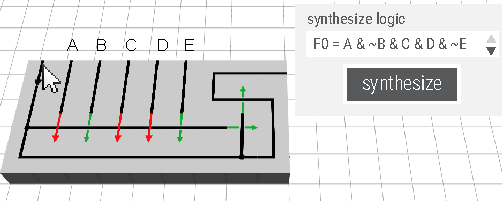
\includegraphics[width=\textwidth]{chapters/digital-metamaterials-FIG/30-editor-synthesize-cells.pdf}
%     \caption[Short figure name.]{Users enter the function `A \& {\textasciitilde}B \& C \& D \& {\textasciitilde}E', and indicates the location by clicking on the grid. Our editor responds by automatically inserting the corresponding cells.
%     \label{fig:30-editor-synthesize-cells}}
% \end{figure}


% \subsection{Implementation}
% We build on the metamaterial mechanisms voxel-style editor and extend it to allow users to draw signal routes and to input logic functions. Our extension of the editor is based on a node.js javascript framework, using the three.js graphics framework and WebGL for rendering the basic geometries.

% Rendering of 3D-printable .stl files was done in modular hierarchical OpenSCAD script files. The editor simply exports the cell geometries as OpenSCAD script commands to render a cell with the specific parameters.

% \subsubsection{Drawing signal paths}
% %\paragraph{Drawing signal paths} 
% Drawing signal paths is realized through a freeform line tool that places appropriately connected cells following the cursor. We use a pathfinding library for 3D\footnote{\url{https://github.com/schteppe/PathFinding3D.js }} that provides the A* pathfinding algorithm to simplify connecting cells via a signal line by finding the shortest available path while crossing existing signals where necessary.

% \subsubsection{Synthesizing cell arrangements}
% %\paragraph{To synthesize cell arrangements}
% To generate cell arrangements of minimal size that implement a user-defined logic function, we use a version of the Espresso heuristic logic minimizer\footnote{\url{https://embedded.eecs.berkeley.edu/pubs/downloads/espresso/index.htm}}. 

% The logic minimizer parses the user text input, minimizes the described input function and returns it in its disjunctive normal form. This minimized DNF is parsed a second time by our editor to identify its terms and literals, which are used to create a very compact cell arrangement that forms a disjunction of minterm conjunctions. A minterm is a minimal conjunction of the input literals that returns true. This means that an array of signals representing the disjunctions of the function is run in parallel. All input variables of the function intersect and potentially block these lines, forming conjunctions along each of the parallel lines. The combined arrangement implements the function as a whole. To choose the most succinct cell representation of the function, we also minimize the negated input function and negate its result again directly on the cell level. The cell arrangement variant that requires the least cells to implement the input function is constructed and placed in the editor at the last user-selected cell location.

% The logic minimizer runs in a separate python virtual environment using the PyEDA\footnote{\url{http://pyeda.readthedocs.io/en/latest/index.html }} library for electronic design automation. This python server is queried via HTTP requests to a REST architecture and replies with minimized functions to logic functions encoded in the request-URL.


\section{Editing digital mechanical metamaterials}

To allow expert users to create and fabricate objects from digital metamaterials, we implemented a specialized 3D voxel-style editor, which is based on the editor for metamaterial mechanisms shown in Section \ref{section:mechanisms-editor}. The main intent is to allow users to draw signal paths and verify them within the editor (Figure \ref{fig:27-editor-interface}). We support users by allowing them to enter simple logic functions, which our editor converts to cell arrangements that implement that function.

While the editor is built to help users design digital metamaterials efficiently, knowledge about signals and logic remains necessary, i.e., this editor is for expert users. 

\begin{figure} [h]
    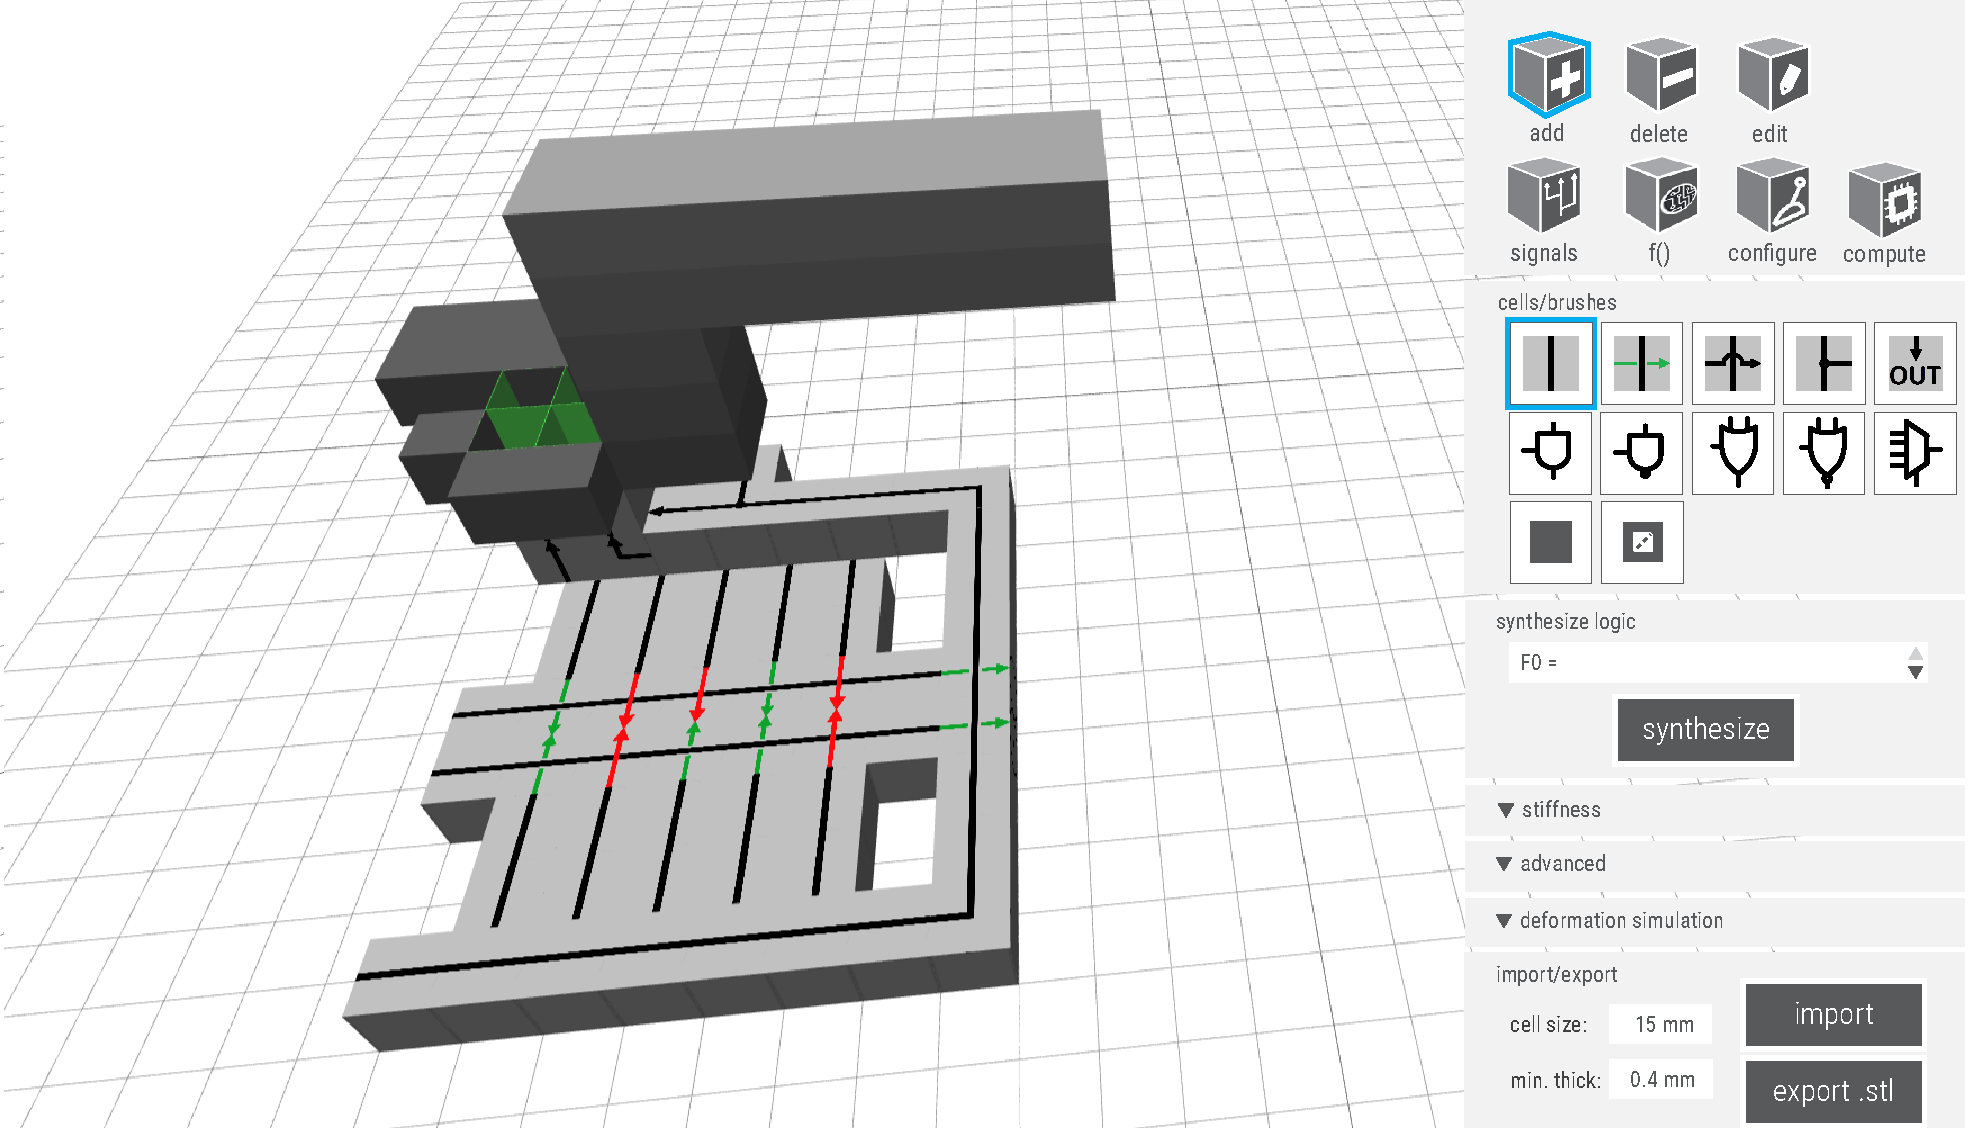
\includegraphics[width=\textwidth]{chapters/digital-metamaterials-FIG/27-editor-interface.pdf}
    \caption[Short figure name.]{Our editor helps users create digital metamaterials.
    \label{fig:27-editor-interface}}
\end{figure}

\subsection{User interaction}
Figure \ref{fig:28-editor-draw-signals} illustrates how users create the door lock example from Figure 1. (a) They first draw the signal line that evaluates the upper 5 digits by dragging over the ground plane using our ``draw signals" tool. (b) Then, using the same tool, they draw signals perpendicular to the first signal line. (c) When the two signals cross, the editor automatically draws a gate cell. (d) They do the same for the lower row of digits. (e) In this example, users manually configure the gate cells using the ``configure", i.e., they change the initial state of 5 gate cells from initially `pass' to `block' by clicking on the respective gate cell. (f) The configured gate cells implement the key code for the lock. 

Users continue by adding the evaluation line, the AND gate and the output cells, which will move the bolts. Finally, they model the analog door latch mechanism on top of the digital metamaterial. 

\begin{figure} [h]
    \includegraphics[width=\textwidth]{chapters/digital-metamaterials-FIG/28-editor-draw-signals.pdf}
    \caption[Short figure name.]{(a) Users draw the signal routing using the ``draw signals" tool. (b) Once they cross an existing signal route, (c) the editor automatically draws a gate cell. (d) After creating all cells for the digit evaluation, (e) users set the initial states of the gate cells using the ``configure" tool (f) to define the key code.
    \label{fig:28-editor-draw-signals}}
\end{figure}

Figure \ref{fig:29-editor-verify-signals} shows how users verify the signal transmission in our custom editor. They first charge the cells by selecting the ``compute" tool. The editor visualizes charged cells by turning the signal lines blue. Clicking on a cell, as shown in Figure \ref{fig:29-editor-verify-signals}a, sets a signal off. The impulse runs through the cells, being visualized in yellow at the currently active cell. After the impulse has passed a cell, the signal path is shown in black again, because the cell is back in its relaxed state (Figure \ref{fig:29-editor-verify-signals}b). To verify the whole computational assembly, users trigger the inputs first and then the evaluation signal, as they do on the 3D printed object. They subsequently watch if the signal runs all the way through to the door. If not, they see where the signal stopped and can correct the error. 

\begin{figure} [h]
    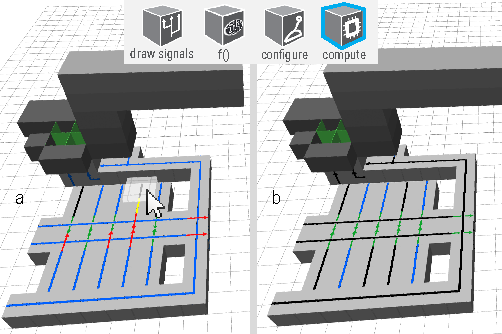
\includegraphics[width=\textwidth]{chapters/digital-metamaterials-FIG/29-editor-verify-signals.pdf}
    \caption[Short figure name.]{Users can verify their logic and signal routing. They first charge all springs, then (a) they click the inputs to trigger the signal there, and lastly (b) they trigger the evaluation line and find that the signal passes all the way through to the latch.
    \label{fig:29-editor-verify-signals}}
\end{figure}

To help users create logic functions efficiently, e.g., by avoiding the need for manual configuration of cells, we allow users to input logic functions. Figure \ref{fig:30-editor-synthesize-cells} shows an example, where users enter the function `A \& {\textasciitilde}B \& C \& D \& {\textasciitilde}E' and click ‘synthesize’. Then, they indicate where the synthesized cell arrangement shall be positioned by simply clicking on the grid. Our editor automatically synthesizes the cells that implement the entered logic functions. 

\begin{figure} [h]
    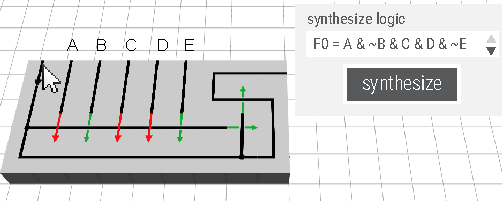
\includegraphics[width=\textwidth]{chapters/digital-metamaterials-FIG/30-editor-synthesize-cells.pdf}
    \caption[Short figure name.]{Users enter the function `A \& {\textasciitilde}B \& C \& D \& {\textasciitilde}E', and indicates the location by clicking on the grid. Our editor responds by automatically inserting the corresponding cells.
    \label{fig:30-editor-synthesize-cells}}
\end{figure}


\subsection{Implementation}
We build on the metamaterial mechanisms voxel-style editor and extend it to allow users to draw signal routes and to input logic functions. Our extension of the editor is based on a node.js javascript framework, using the three.js graphics framework and WebGL for rendering the basic geometries.

Rendering of 3D-printable .stl files was done in modular hierarchical OpenSCAD script files. The editor simply exports the cell geometries as OpenSCAD script commands to render a cell with the specific parameters.

\subsubsection{Drawing signal paths}
%\paragraph{Drawing signal paths} 
Drawing signal paths is realized through a freeform line tool that places appropriately connected cells following the cursor. We use a pathfinding library for 3D\footnote{\url{https://github.com/schteppe/PathFinding3D.js}} that provides the A\* pathfinding algorithm to simplify connecting cells via a signal line by finding the shortest available path while crossing existing signals where necessary.


\subsection{Synthesizing cell arrangements from boolean expressions}
%\paragraph{To synthesize cell arrangements}
To generate cell arrangements of minimal size that implement a user-defined logic function, we use a version of the Espresso heuristic logic minimizer\footnote{\url{https://embedded.eecs.berkeley.edu/pubs/downloads/espresso/index.htm}}. 

The logic minimizer parses the user text input, minimizes the described input function and returns it in its disjunctive normal form. This minimized DNF is parsed a second time by our editor to identify its terms and literals, which are used to create a very compact cell arrangement that forms a disjunction of minterm conjunctions. A minterm is a minimal conjunction of the input literals that returns true. This means that an array of signals representing the disjunctions of the function is run in parallel. All input variables of the function intersect and potentially block these lines, forming conjunctions along each of the parallel lines. The combined arrangement implements the function as a whole. To choose the most succinct cell representation of the function, we also minimize the negated input function and negate its result again directly on the cell level. The cell arrangement variant that requires the least cells to implement the input function is constructed and placed in the editor at the last user-selected cell location.

The logic minimizer runs in a separate python virtual environment using the PyEDA\footnote{\url{http://pyeda.readthedocs.io/en/latest/index.html }} library for electronic design automation. This python server is queried via HTTP requests to a REST architecture and replies with minimized functions to logic functions encoded in the request-URL.

%\subsection{Simulating signal flow}



\section{Conclusions}

We presented digital mechanical metamaterials. While (analog) metamaterial mechanisms suffer from signal decay, digital metamaterials are not subject to such decay, allowing us to create larger or more complex objects. Unlike solutions based on sensors, actuators, and microcontrollers, our approach still is entirely mechanical. 

We showed the design of bit cells, which are the key element for the signal transmission. They contain bistable springs, which have two states, the relaxed and tense state. We also presented cells that allow for routing signals in 2D and 3D. To employ simple computation, we showed gate cells. We demonstrated our approach at the example of two prototypes: a digital door lock without electronics and a configurable plant pot. To help expert users create such digital metamaterials, we contribute an editor that allows for routing signals, verifying them, and synthesizing cell arrangements from user-defined logic functions.

%For future work, we plan to explore cells that have the ability to shear and transmit signals, which would allow us to change the properties of every single cell within an object.


%Acknowledgements
%We want to thank David Lindlbauer, Pedro Lopes, Stefanie Müller, and Willi Müller for their help and feedback.


% \section{Editor: adding computation to 3D objects}
